\documentclass[10pt]{article}
\usepackage[utf8]{inputenc}
\usepackage[T1]{fontenc}
\usepackage[a4paper,margin=0.9in]{geometry}
\usepackage{amsmath,amssymb,amsfonts}
\usepackage{array,booktabs,tabularx}
\usepackage{graphicx}
\graphicspath{{../results/}}
\usepackage{tikz}
\usetikzlibrary{arrows.meta,positioning,shapes.geometric}
\usepackage{lmodern}
\usepackage{microtype}
\setlength{\parindent}{0pt}
\setlength{\parskip}{0.5em}
\renewcommand{\arraystretch}{1.12}

\title{PGMO Invited Course Report}
\author{Xiangyu LUO}
\date{April 2026}

\begin{document}
\maketitle

\section{Introduction}

High-dimensional convex geometry studies how volume and probability distribute on convex bodies after the correct normalization. For uniform measures on convex sets, and more generally for isotropic log-concave measures on $\mathbb{R}^n$, many quantities that look unstable in low dimension become sharply regular in high dimension: mass concentrates, many one-dimensional marginals are close to Gaussian, and central sections obey strong comparison principles. A natural way to organize this subject is through three closely related questions: the thin-shell problem, Bourgain's slicing problem, and the Kannan--Lov\'asz--Simonovits (KLS) conjecture.

These questions are important because they connect geometric information, probabilistic behavior, and analytic inequalities. The thin-shell problem asks for quantitative radial concentration, the slicing problem asks how much mass must remain visible in codimension one, and KLS asks for a full dimension-free Poincar\'e or isoperimetric theory for isotropic log-concave measures. The modern picture combines concentration of measure, log-concavity, Bochner identities, negative Sobolev norms, optimal transport, and stochastic localization. It also points toward broader applications in high-dimensional probability and quantitative functional inequalities.

\section{Background and Main Problems}

\subsection{Geometric Models and Isotropic Position}

The cube, the Euclidean ball, and the sphere already display the main geometric scale of the subject. In dimension $n$, the relevant length is typically $\sqrt{n}$ rather than a fixed Euclidean size. In the cube $[-1/2,1/2]^n$, the distance between two independent random points is concentrated around a multiple of $\sqrt{n}$. For the Euclidean ball and sphere, the same scale appears after the natural normalization. These examples suggest a general principle: in high dimension, mass is often concentrated in thin regions, and geometric quantities become predictable once the right normalization is chosen.

The sphere gives the cleanest first model of this phenomenon. Most of its mass lies near an equator, and more generally near the boundary of any set whose measure is neither very small nor very close to one. This is the geometric content behind concentration of measure and L\'evy's spherical isoperimetric inequality. It shifts attention from raw volume estimates to the behavior of Lipschitz observables, neighborhoods, random projections, and typical sections.

The standard normalization is isotropic position. A random vector $X$ is isotropic when
\[
\mathbb{E}X=0, \qquad \mathrm{Cov}(X)=I_n.
\]
This removes irrelevant affine distortions and fixes the ambient scale. After isotropic normalization, every marginal $\langle X,\theta\rangle$ has mean zero and variance one, while the Euclidean norm $|X|$ is centered near $\sqrt{n}$. In this form, the main conjectures and theorems can be compared directly across different convex bodies and log-concave measures.

The cube and the sphere also reveal two complementary mechanisms behind concentration. In the cube, concentration comes from independence of coordinates and classical inequalities of Bernstein or Hoeffding type. On the sphere, and more generally in convex settings, concentration is produced by geometry itself. The general theory of log-concave measures can be read as a framework in which these two viewpoints meet.

\subsection{Thin-Shell, Slicing, and KLS}

The subject is organized around three benchmark problems in asymptotic convex geometry. They are related, but each emphasizes a different form of regularity.

\begin{center}
\begin{tabularx}{0.98\textwidth}{>{\raggedright\arraybackslash}p{0.2\textwidth} >{\raggedright\arraybackslash}X >{\raggedright\arraybackslash}p{0.2\textwidth}}
\toprule
Problem & Formulation in isotropic position & Why it matters \\
\midrule
Thin-shell problem & Whether an isotropic log-concave $X$ satisfies $\mathrm{Var}(|X|^2)\leq Cn$, equivalently whether the mass is concentrated near the radius $\sqrt{n}$ with shell width of order one & It measures radial concentration and controls the emergence of Gaussian marginals \\
\addlinespace
Bourgain's slicing problem & Whether every volume-one convex body has a central hyperplane section with $(n-1)$-dimensional volume bounded below by a universal constant; equivalently, whether the isotropic constant is universally bounded & It asks for a dimension-free section estimate in codimension one \\
\addlinespace
KLS conjecture & Whether every isotropic log-concave measure satisfies a dimension-free Poincar\'e or isoperimetric inequality for all sufficiently regular observables & It is the strongest expected form of dimension-free spectral and isoperimetric control \\
\bottomrule
\end{tabularx}
\end{center}

The thin-shell problem concerns the fluctuations of the Euclidean norm. Its standard form asks whether
\[
\mathrm{Var}(|X|^2)\leq Cn
\]
for every isotropic log-concave random vector $X$ in $\mathbb{R}^n$. Since $\mathbb{E}|X|^2=n$, this means that most of the mass should lie in a shell of bounded width around the radius $\sqrt{n}$. The problem is important because radial concentration has consequences far beyond the norm itself, especially for the normal approximation of one-dimensional marginals.

Bourgain's slicing problem is more geometric. It asks for a universal lower bound on the volume of a central hyperplane section of any volume-one convex body. Although this question is formulated in terms of sections, it turns out to be closely connected with the same isotropic and probabilistic structure that governs thin shells. A radial statement about $|X|$ can therefore have strong consequences for codimension-one geometry.

The Kannan--Lov\'asz--Simonovits conjecture \cite{KLS95} is stronger than both. In one standard form, it predicts that
\[
\mathrm{Var}(f(X))\leq C\,\mathbb{E}|\nabla f(X)|^2
\]
for every sufficiently regular observable $f$ under an isotropic log-concave law. This is not a bound for one special function such as $|x|^2$; it is a dimension-free spectral or isoperimetric statement for all observables. The recent thin-shell bound establishes this inequality only for the particular choice $f(x)=|x|^2$, so KLS remains the natural open endpoint of the theory.

\section{Main Methods and Main Theorem}

\subsection{Concentration and the Thin-Shell Theorem}

The first step is to understand why Gaussian behavior appears so often in high dimension. On the sphere, Lipschitz functions are strongly concentrated around a central value, with fluctuations of size roughly $1/\sqrt{n}$. This means that regular observables on high-dimensional spheres are nearly constant, and it explains why typical projections and sections often behave as if a Gaussian law were present in the background.

The thin-shell theorem, i.e.\ the central limit theorem for convex sets \cite{ABP03,Kla07}, makes this link explicit. In a simplified form, it says that if an isotropic random vector $X$ satisfies
\[
\mathbb{E}\left(\frac{|X|}{\sqrt{n}}-1\right)^2\leq \varepsilon^2,
\]
then for most directions $\theta\in S^{n-1}$ the marginal $\langle X,\theta\rangle$ is close to the standard Gaussian law. The theorem separates two tasks that should be distinguished: first establish radial concentration, and then deduce Gaussian marginals from that concentration. The second step is geometric and probabilistic; the first requires deeper structure.

Examples clarify the content of this theorem. Independent coordinates with bounded fourth moments satisfy the thin-shell assumption, so the result is consistent with the classical central limit phenomenon. A regular simplex is far less symmetric than the cube or the ball and its vertices lie on a sphere, but the uniform measure on the solid simplex in isotropic position still satisfies a thin-shell bound and has approximately Gaussian marginals in most directions (see the simulation below). By contrast, a mixture of two spheres of very different radii is isotropic but not thin-shell, and its marginals are far from Gaussian. The message is that isotropicity alone is not enough: what matters is the radial organization of the mass.

\subsection{Log-Concavity and the Bochner Framework}

The natural class for the general theory is the class of log-concave measures. A density $\rho$ is log-concave when $-\log\rho$ is convex on its support. This includes uniform measures on convex bodies and Gaussian measures, and it is stable under the operations that matter most in geometry and probability: projections, linear images, convolutions, and weak limits. The Pr\'ekopa--Leindler inequality is the key tool behind this stability, and it plays the role of a functional Brunn--Minkowski inequality.

Log-concavity already gives strong one-dimensional information. An isotropic log-concave random variable has a density bounded below near the origin and exponential decay at infinity, and its moments satisfy reverse H\"older-type comparisons. These facts imply, for instance, that central hyperplane sections of an isotropic convex body are comparable up to universal constants. The background geometry is therefore already highly constrained before the sharp thin-shell bound enters.

The analytic framework is built from Bochner's method. Writing the density as $d\mu=e^{-\psi(x)}dx$, one introduces the weighted operator
\[
L u=\Delta u-\nabla\psi\cdot\nabla u.
\]
This operator is symmetric in $L^2(\mu)$, and the Hessian $\nabla^2\psi$ plays the role of a curvature term. The integrated Bochner identity takes the form
\[
\int (Lu)^2\,d\mu
=\int (\nabla^2\psi\,\nabla u)\cdot\nabla u\,d\mu
+\int \|\nabla^2u\|_{HS}^2\,d\mu.
\]
Since $\psi$ is convex, the first term on the right is nonnegative, so convexity produces direct analytic control.

This viewpoint is then dualized through the negative Sobolev norm $H^{-1}(\mu)$. For a mean-zero function $f$, the norm $\|f\|_{H^{-1}(\mu)}$ measures how large $\int f u\,d\mu$ can be when the Dirichlet energy of $u$ is bounded. The resulting inequality
\[
\mathrm{Var}_{\mu}(f)\leq \sum_{i=1}^n \|\partial_i f\|_{H^{-1}(\mu)}^2
\]
turns variance estimates into statements about infinitesimal transport and differential structure. This is the key transition from qualitative convexity to quantitative control of fluctuations.

\subsection{Transport, Gaussian Tilts, and Brownian Coupling}

The recent main theorem of Klartag and Lehec \cite[Theorem~1.1]{KL25} states that for every isotropic log-concave random vector $X$ in $\mathbb{R}^n$,
\[
\mathrm{Var}(|X|^2)\leq Cn.
\]
Consequently,
\[
\mathbb{E}(|X|-\sqrt{n})^2\leq C.
\]
This is the sharp thin-shell bound up to the value of the universal constant. It is not only a radial statement: through the implication from thin shell to slicing \cite{EK11}, it gives a new proof of Bourgain's slicing theorem, which had been established shortly before by Klartag and Lehec using Guan's bound \cite{Gua24,KL24}.

The proof does not estimate $\mathrm{Var}(|X|^2)$ directly. Instead, it reduces the problem to an $H^{-1}$ estimate for coordinate functions, namely
\[
\sum_{i=1}^n \|x_i\|_{H^{-1}(\mu)}^2\leq Cn
\]
for every isotropic log-concave probability measure $\mu$. At this point, the transport interpretation of $H^{-1}(\mu)$ becomes essential:
\[
\|f\|_{H^{-1}(\mu)}
\leq \liminf_{\varepsilon\to 0^+}
\frac{W_2\bigl(\mu,(1+\varepsilon f)\mu\bigr)}{\varepsilon}.
\]
This reformulates a variance estimate as a problem about the cost of infinitesimal deformations of the measure.

The next ingredient is a family of localized Gaussian tilts,
\[
p_{t,y}(x)=\exp\!\left( y\cdot x-\frac{t|x|^2}{2}-\Lambda_t(y)\right)p(x),
\]
where $p$ is the original density and $\Lambda_t$ is the corresponding log-Laplace normalizing factor. These tilted measures remain uniformly log-concave at scale $t$, so the convexity tools remain available along the deformation. Their barycenters and covariance matrices,
\[
a_t(y)=\nabla\Lambda_t(y), \qquad A_t(y)=\nabla^2\Lambda_t(y),
\]
become the central dynamical quantities.

The last step is a Brownian or pathwise coupling of these tilts, in the spirit of Eldan's stochastic localization \cite{Eld13}; Klartag and Lehec call their version parallel coupling \cite{KL25}. Instead of studying the deformation only through partial differential equations, one follows a stochastic process of the form
\[
\theta_t=\theta_0+w_t+\int_0^t a_s(\theta_s)\,ds,
\]
with Brownian driving path $w_t$ in the main application. Along this evolution, the covariance matrices $A_t$ satisfy structural bounds such as $A_t\leq t^{-1}I$. The decisive issue is not whether a single eigenvalue can become large, but whether many eigenvalues can be simultaneously large. Quantitative eigenvalue control, combined with estimates on the derivative flow, closes the $H^{-1}$ bound and therefore the thin-shell estimate.

\begin{center}
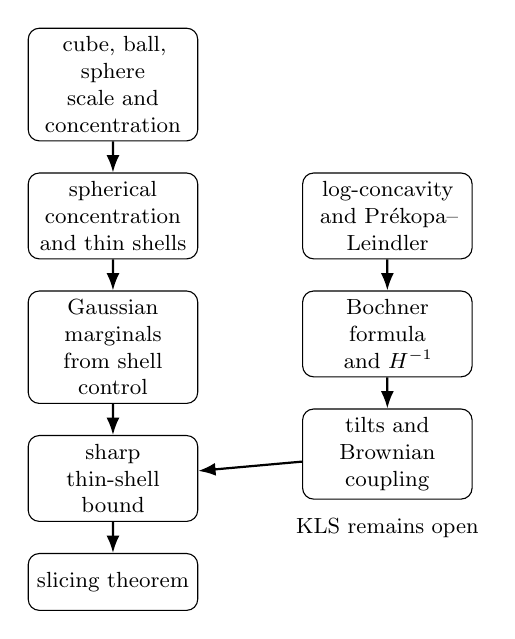
\begin{tikzpicture}[
scale=0.88,
transform shape,
node distance=0.45cm and 0.55cm,
box/.style={draw, rounded corners, align=center, minimum height=0.82cm, text width=2.2cm, inner sep=3.5pt, font=\small},
arrow/.style={-{Latex[length=2.2mm]}, thick}
]
\node[box] (examples) {cube, ball, sphere\\scale and concentration};
\node[box, below=of examples] (concentration) {spherical concentration\\and thin shells};
\node[box, right=1.5cm of concentration] (logconc) {log-concavity\\and Pr\'ekopa--Leindler};
\node[box, below=of concentration] (gaussian) {Gaussian marginals\\from shell control};
\node[box, below=of logconc] (bochner) {Bochner formula\\and $H^{-1}$};
\node[box, below=of bochner] (tilts) {tilts and\\Brownian coupling};
\node[box, below=of gaussian] (shell) {sharp\\thin-shell bound};
\node[box, below=of shell] (slicing) {slicing theorem};
\node[align=center, font=\small, below=0.15cm of tilts] (kls) {KLS remains open};

\draw[arrow] (examples) -- (concentration);
\draw[arrow] (concentration) -- (gaussian);
\draw[arrow] (logconc) -- (bochner);
\draw[arrow] (bochner) -- (tilts);
\draw[arrow] (tilts) -- (shell);
\draw[arrow] (gaussian) -- (shell);
\draw[arrow] (shell) -- (slicing);
\end{tikzpicture}
\end{center}

This scheme summarizes the global logic. Geometric concentration explains why thin shells matter and why they imply Gaussian marginals, while log-concavity, Bochner estimates, transport, and Brownian coupling supply the mechanism behind the sharp shell bound. Slicing follows as a consequence, and KLS remains the broader unresolved direction.

\subsection{A Numerical Illustration}

The thin-shell statement can be observed directly by simulation (script \texttt{thin\_shell\_demo.py}). We sample uniformly from three convex bodies put in isotropic position --- the cube $[-\sqrt3,\sqrt3]^n$, the ball of radius $\sqrt{n+2}$, and the regular simplex --- and from an isotropic but non-log-concave measure, the equal mixture of $N(0,s_1^2I_n)$ and $N(0,s_2^2I_n)$ with $s_1^2=0.25$ and $s_2^2=1.75$. With $20\,000$ samples (5\,000 for $n=1000$), the normalized fluctuation $\mathrm{Var}(|X|^2)/n$ is

\begin{center}
\begin{tabular}{lccccc}
\toprule
& $n=10$ & $n=30$ & $n=100$ & $n=300$ & $n=1000$\\
\midrule
cube & 0.79 & 0.79 & 0.80 & 0.79 & 0.80\\
ball & 0.29 & 0.11 & 0.039 & 0.013 & 0.004\\
simplex & 2.68 & 3.32 & 3.77 & 3.88 & 3.95\\
Gaussian mixture & 8.6 & 20.0 & 59.7 & 171.7 & 563.2\\
\bottomrule
\end{tabular}
\end{center}

For the three convex bodies the ratio stays bounded, in agreement with $\mathrm{Var}(|X|^2)\le Cn$: for the cube it equals $\mathbb E X_1^4-1=0.8$ exactly, for the ball it even decays like $4/n$, and for the simplex it tends to $4$, the value predicted by its representation through normalized exponential variables. For the mixture it grows linearly in $n$, i.e.\ $\mathrm{Var}(|X|^2)\asymp n^2$, because $|X|/\sqrt n$ concentrates around two different radii. Figure~\ref{fig:thin-shell} also shows a random one-dimensional marginal in dimension $1000$: it is indistinguishable from $N(0,1)$ for the three bodies and visibly non-Gaussian for the mixture, which is the dichotomy described by the thin-shell theorem.

\begin{figure}[h]
\centering
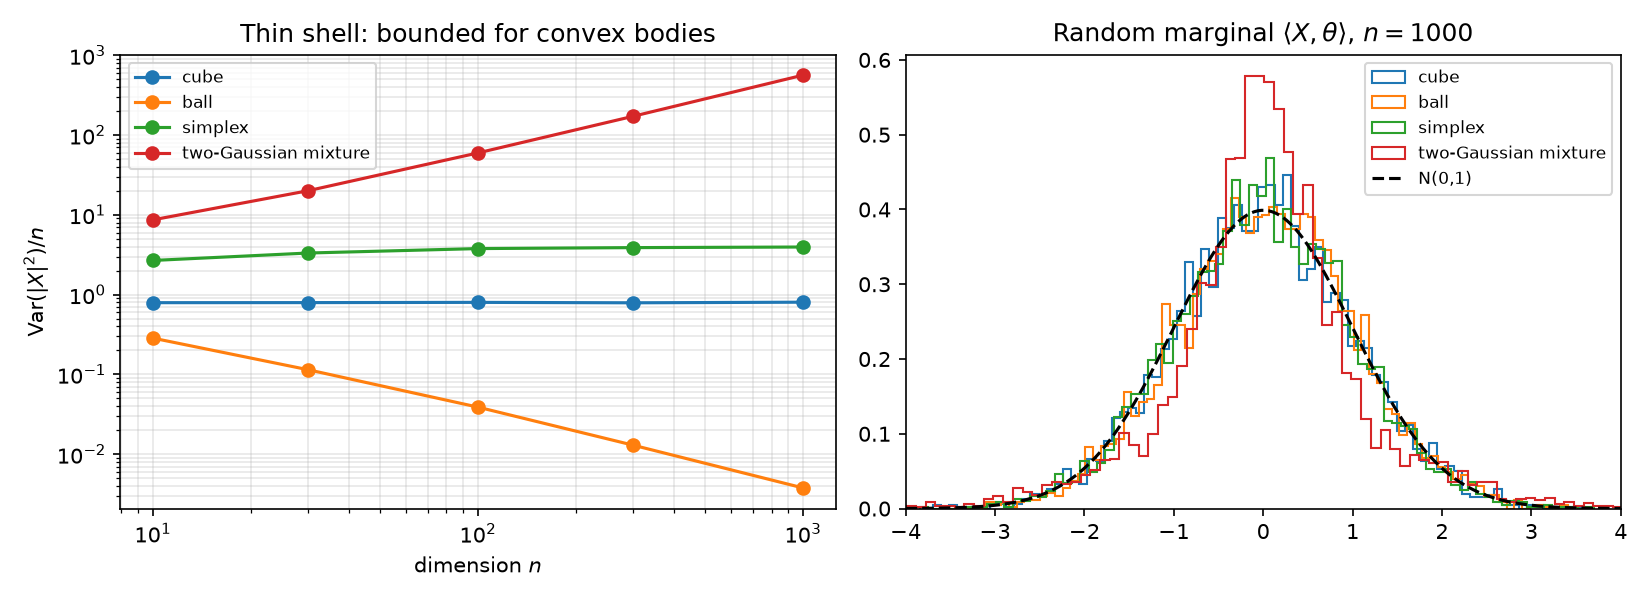
\includegraphics[width=\linewidth]{thin_shell.png}
\caption{Left: $\mathrm{Var}(|X|^2)/n$ as a function of the dimension. Right: histogram of $\langle X,\theta\rangle$ for a random direction $\theta$ in dimension $1000$.}
\label{fig:thin-shell}
\end{figure}

\section{Main Results}

The principal result is the sharp thin-shell bound for isotropic log-concave measures. It shows that the mass is confined to a shell of bounded width around the radius $\sqrt{n}$, uniformly in the dimension. Beyond radial concentration, this yields an affirmative solution to Bourgain's slicing problem through known geometric implications.

Another important conclusion is methodological. The proof combines geometric concentration, the stability theory of log-concavity, Bochner-type curvature estimates, negative Sobolev norms, transport inequalities, and stochastic localization. The result is therefore valuable not only as a theorem, but also as a synthesis of several modern methods in high-dimensional convex geometry.

\begin{thebibliography}{KLS95}\small
\bibitem[ABP03]{ABP03} M.~Anttila, K.~Ball, I.~Perissinaki. The central limit problem for convex bodies. \emph{Trans. Amer. Math. Soc.} 355 (2003), 4723--4735.
\bibitem[EK11]{EK11} R.~Eldan, B.~Klartag. Approximately Gaussian marginals and the hyperplane conjecture. \emph{Contemp. Math.} 545 (2011), 55--68.
\bibitem[Eld13]{Eld13} R.~Eldan. Thin shell implies spectral gap up to polylog via a stochastic localization scheme. \emph{Geom. Funct. Anal.} 23 (2013), 532--569.
\bibitem[Gua24]{Gua24} Q.~Guan. A note on Bourgain's slicing problem. arXiv:2412.09075, 2024.
\bibitem[Kla07]{Kla07} B.~Klartag. A central limit theorem for convex sets. \emph{Invent. Math.} 168 (2007), 91--131.
\bibitem[KL24]{KL24} B.~Klartag, J.~Lehec. Affirmative resolution of Bourgain's slicing problem using Guan's bound. arXiv:2412.15044, 2024.
\bibitem[KL25]{KL25} B.~Klartag, J.~Lehec. Thin-shell bounds via parallel coupling. arXiv:2507.15495, 2025.
\bibitem[KLS95]{KLS95} R.~Kannan, L.~Lov\'asz, M.~Simonovits. Isoperimetric problems for convex bodies and a localization lemma. \emph{Discrete Comput. Geom.} 13 (1995), 541--559.
\end{thebibliography}

\end{document}
